\documentclass[11pt,a4paper]{article}

% ---------------- Layout & typography --------------------------------
\usepackage[a4paper,margin=1in]{geometry}
\usepackage{mathptmx}              % Times-like serif, widely available
\usepackage[T1]{fontenc}
\usepackage{microtype}
\usepackage{setspace}
\onehalfspacing
\usepackage{enumitem}
\setlist{noitemsep,topsep=2pt}

% ---------------- Tables & misc --------------------------------------
\usepackage{booktabs}
\usepackage{array}
\usepackage{graphicx}
\graphicspath{{figures/}}
\usepackage{placeins}
\renewcommand{\topfraction}{0.9}
\renewcommand{\bottomfraction}{0.8}
\renewcommand{\textfraction}{0.07}
\renewcommand{\floatpagefraction}{0.8}
\usepackage{amsmath,amssymb}
\usepackage[hidelinks]{hyperref}
\usepackage{titlesec}
\titleformat{\section}{\normalfont\large\bfseries}{\thesection}{0.6em}{}
\titleformat{\subsection}{\normalfont\normalsize\bfseries}{\thesubsection}{0.6em}{}
\titlespacing*{\section}{0pt}{12pt plus 2pt minus 2pt}{4pt}
\titlespacing*{\subsection}{0pt}{8pt plus 2pt minus 2pt}{3pt}

\setlength{\parskip}{4pt plus 1pt minus 1pt}
\setlength{\parindent}{0pt}

% =====================================================================
\begin{document}

% ---------------- Title block ----------------------------------------
\begin{center}
  {\Large\bfseries Toward Industrially Deployable Multi-Agent\\[2pt]
   Reinforcement-Learning Control of Virtual Synchronous Generators}\\[10pt]
  {\normalsize Research Proposal for the Master by Research (MRes)}\\[2pt]
  {\normalsize Department of Electrical and Electronic Engineering,
   University of Nottingham Ningbo China}\\[6pt]
  {\normalsize Yuang Wei \quad$\cdot$\quad Intended supervisor: Dr John Xu
   \quad$\cdot$\quad 2026}
\end{center}
\vspace{4pt}
\hrule
\vspace{8pt}

% =====================================================================
\section{Introduction}

The decarbonisation of electricity supply is replacing conventional
synchronous generators with inverter-based renewable
resources~\cite{iea_renewables_2024}. Because inverters do not couple a
rotating mass to the grid, this shift erodes the physical inertia that
damps frequency excursions after a generation--load imbalance.
Low-inertia systems then show faster frequency dynamics and larger rates
of change of frequency, a recognised threat to stable
operation~\cite{tielens2016inertia,milano2018foundations,markovic2021lowinertia}.

\emph{Virtual synchronous generators} (VSGs) are a leading remedy: they
program grid-connected power electronics to emulate the
electromechanical swing dynamics of a synchronous machine; the emulation exposes a
virtual inertia and a virtual damping coefficient that shape the
frequency response~\cite{zhong2011vsg,beck2007vsg,darco2015vsm}. In
conventional designs these parameters are fixed at commissioning, yet
their optimal values depend on the operating point, the load
composition, and the disturbance, so a fixed-parameter VSG is
sub-optimal under variable renewable-grid
conditions~\cite{bevrani2014vsg}. The direct response is to adapt these parameters online and, when
several VSGs operate in parallel, to coordinate them across units.

Reinforcement learning (RL) is the dominant data-driven route to such
adaptive coordination, and the applicant has built a large body of work
mapping what multi-agent RL can and cannot do on this problem
(Section~3). In that work the applicant identified a concrete obstacle
to real-world use: a learned controller must be trained at length for
one specific network, and that training does not transfer to the many
topologies a utility operates. The proposed MRes addresses the question
this raises: can multi-agent RL control of paralleled VSGs be made
topology-general and deployable, effective across different grid
configurations without per-network retraining, and where it cannot, when
should classical control be preferred?

% =====================================================================
\section{Literature Review}

Ernst~\emph{et~al.}\ first applied RL to power-system control,
comparing fitted-Q iteration against model predictive
control~\cite{ernst2009rl}; Hadidi~\emph{et~al.}\ extended it to
wide-area stabilisation~\cite{hadidi2013ml}, and
Glavic~\emph{et~al.}\ surveyed the field~\cite{glavic2017rl}.
The continuous-action methods
relevant to VSG tuning descend from the deep deterministic policy
gradient~\cite{lillicrap2016ddpg} and its successors, twin-delayed DDPG
(TD3)~\cite{fujimoto2018td3} and soft actor--critic
(SAC)~\cite{haarnoja2018sac}; coordinating several controllers draws on
centralised-training, decentralised-execution multi-agent
actor--critic methods~\cite{lowe2017maddpg}. The most direct prior art
is Yang~\emph{et~al.}~\cite{yang2023ddic}, who govern four paralleled
VSGs with independent SAC agents on the modified Kundur four-machine
benchmark~\cite{kundur1994power,klein1991study} and report gains over a
tuned adaptive baseline (Figure~\ref{fig:arch}). Across this literature one
question stays contested: whether the gains of learning-based control
justify its opacity and per-network training cost over a well-tuned
classical droop controller, which remains the deployed
standard~\cite{bevrani2014vsg}.

\begin{figure}[t]
  \centering
  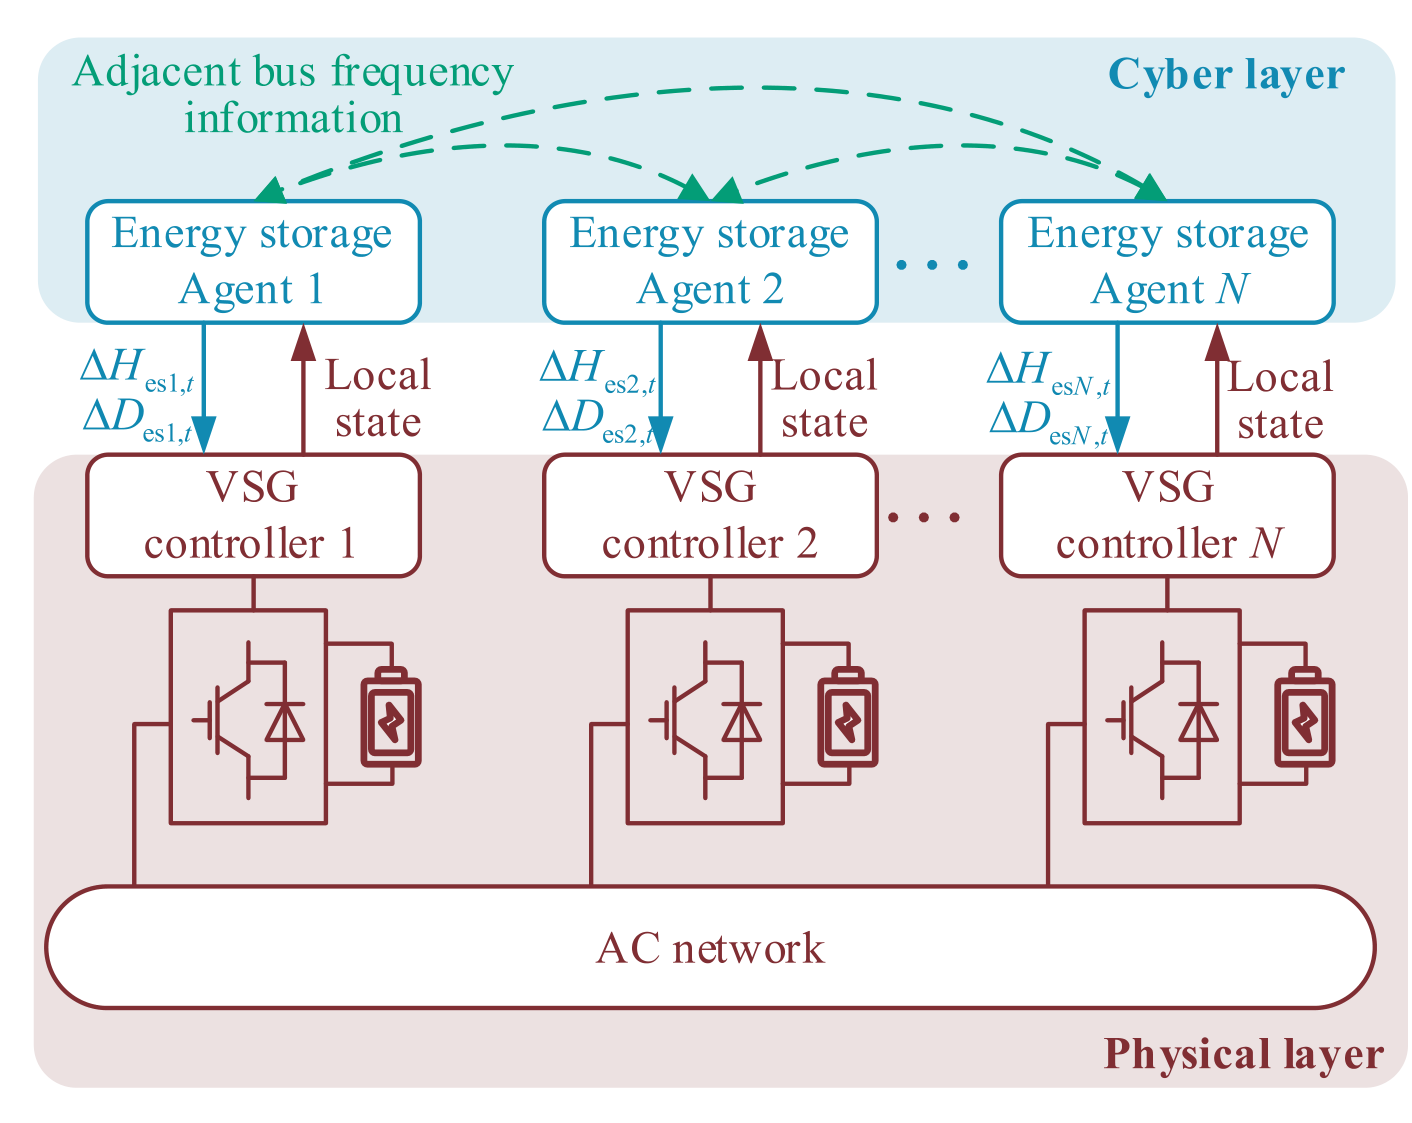
\includegraphics[width=0.70\linewidth]{paper_fig1_architecture}
  \caption{Distributed multi-agent control architecture for paralleled
  VSGs: each energy-storage agent sets the virtual inertia $\Delta H$ and
  damping $\Delta D$ of its converter from local state and
  neighbouring-bus frequency exchanged over a fault-prone communication
  layer. Source: Yang \emph{et al.}~\cite{yang2023ddic}.}
  \label{fig:arch}
\end{figure}

The proposed work addresses three gaps. First, deep-RL controllers are
sensitive to random seed and early
training~\cite{henderson2018deepreinforcement}, and reproducibility-aware
reporting~\cite{agarwal2021precipice} remains rare in power-system RL.
Second, and most important for deployment, these controllers are trained
per network: a policy learned on one topology has no principled
way to transfer to another, so the training cost recurs for every
configuration a utility operates. Third, graph neural networks (GNNs),
which operate on the network as a graph, have shown promise for
topology-aware power-system
learning~\cite{owerko2020opfgnn,liao2022gnnreview}, but have not, to the
applicant's knowledge, been applied to make multi-agent VSG inertia and
damping control transferable across topologies. The proposed work sets out to close that gap.

% =====================================================================
\section{Preliminary Work and Demonstrated Capability}

The applicant has already carried out extensive prior work on this
problem, beginning with a
final-year project that reproduced the multi-agent SAC controller
of~\cite{yang2023ddic} for four paralleled VSGs on the modified Kundur
network, using the open-source ANDES phasor-domain
simulator~\cite{cui2021andes} as a fully programmable, Python-native
training environment. Since then the applicant has extended that work into a sustained research programme\footnote{The complete codebase, experiment ledger, and audited claim records are publicly available at \url{https://github.com/wya5217799/andes-rl-kundur}.}:

\begin{center}\small
\begin{tabular}{@{}r@{\quad}l@{\qquad}r@{\quad}l@{}}
\textbf{259} & experimental rounds (R01--R259) &
\textbf{12} & deep-RL algorithm variants \\
\textbf{263} & audited, traceable findings &
\textbf{91} & training trials mapping the plateau \\
\textbf{35+} & automated regression tests &
\textbf{16-pp} & manuscript in IEEE journal format \\
\end{tabular}
\end{center}

The experimental framework is a layered, reproducible pipeline:
\begin{itemize}
  \item \textit{Scenario layer:} the modified Kundur network and a fixed
        set of load-disturbance test cases (the LS1/LS2 load steps
        of~\cite{yang2023ddic}), held constant so that every controller
        faces identical disturbances.
  \item \textit{Simulation layer:} the ANDES phasor-domain
        solver~\cite{cui2021andes} wrapped as a reinforcement-learning
        environment; each training and evaluation step advances a
        time-domain power-system simulation, so an agent learns against
        the grid's own dynamics.
  \item \textit{Algorithm layer:} the multi-agent controllers of
        Table~\ref{tab:algos}, interchangeable behind a common
        interface.
  \item \textit{Evaluation layer:} two scorers applied to the saved
        trajectories: the eleven-axis paper-grade metric (the project's
        multi-dimensional score) and the paper-faithful cumulative
        frequency-deviation reward of~\cite{yang2023ddic}, which places
        each agent on the reference paper's own scale.
\end{itemize}
A single run proceeds train, test, score: an agent is trained online
against the simulator; the saved checkpoint is replayed on the fixed
disturbance scenarios with learning switched off; and the recorded
traces are scored on both metrics and ranked against the no-control and
classical-droop baselines.

The applicant implemented twelve distinct controller
designs and compared them directly on the same
benchmark and evaluation protocol (Table~\ref{tab:algos}), spanning the
SAC and TD3 families, recurrent (LSTM) and distributional
(quantile-regression) critics, adaptive feature extraction, and a
Transformer actor.

\begin{table}[t]
  \centering\small
  \caption{The twelve deep-RL controller variants implemented and
           compared for multi-agent VSG inertia/damping control on the
           modified Kundur benchmark.}
  \label{tab:algos}
  \renewcommand{\arraystretch}{1.15}
  \begin{tabular}{@{}p{3.0cm}p{6.1cm}p{5.3cm}@{}}
    \toprule
    \textbf{Variant} & \textbf{Function / innovation tested} &
    \textbf{Outcome} \\
    \midrule
    SAC & Reference paper's multi-agent algorithm~\cite{yang2023ddic}
        & Reproduced; reference behaviour. \\
    SAC--CTDE & Centralised-training, decentralised-execution critic
        & No gain beyond the plateau band. \\
    TD3 & Twin-delayed deterministic policy gradient
        & Stable deterministic baseline. \\
    TD3--LSTM & Recurrent actor with memory of recent states
        & Strongest single family; the SOTA base. \\
    TD3--LSTM2 & Deeper two-layer recurrence
        & Within the plateau band. \\
    TD3--LSTM--hreg & Hidden-state regularisation
        & Improved stability; within band. \\
    TD3--LSTM--warmh0 & Warm hidden-state initialisation
        & Mitigated seed collapse; partial. \\
    TD3--QR--LSTM & Distributional quantile-regression critic
        & Matched the LSTM SOTA. \\
    TD3--QR--LSTM--hreg & Distributional critic + hidden-state reg.
        & Within band. \\
    TD3--AFE--LSTM & Adaptive feature-extraction front-end
        & Within band. \\
    TD3--QR--AFE--LSTM & Combined distributional + adaptive features
        & Within band. \\
    TD3--Transformer & Attention-based actor over a rolling window
        & Negative result: deterministic-eval collapse. \\
    \bottomrule
  \end{tabular}
\end{table}

\begin{figure}[t]
  \centering
  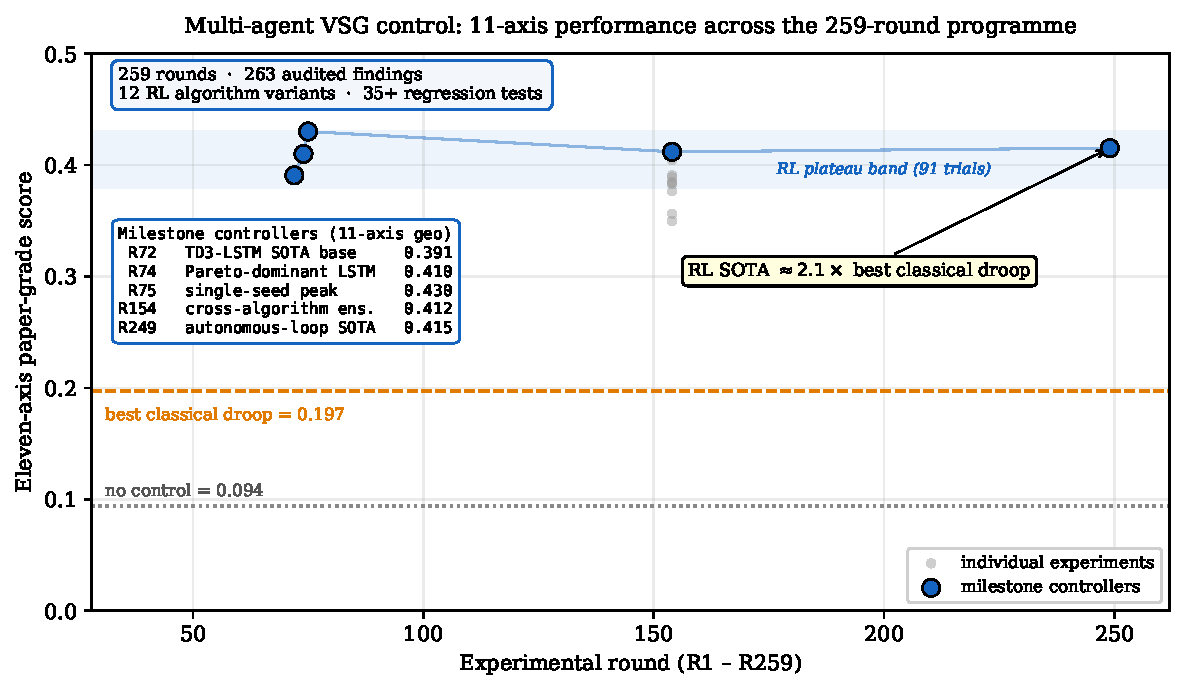
\includegraphics[width=0.88\linewidth]{proposal_progression}
  \caption{Eleven-axis paper-grade score of the milestone multi-agent
  controllers across the 259-round research programme, set against the
  no-control and best classical-droop baselines. The learning-based
  controllers cluster in a structural performance plateau roughly
  $2.1\times$ above the best tuned classical droop controller; every
  plotted value is pinned to an audited claim in the project ledger
  (author's own work).}
  \label{fig:progression}
\end{figure}

(1) The applicant developed a purpose-built eleven-axis
paper-grade evaluation metric to expose single-axis
failure modes that a scalar reward conceals. (2) Across all twelve
variants, single-algorithm performance clustered in a narrow band
(roughly $0.38$--$0.43$ on the eleven-axis score; Figure~\ref{fig:progression}); (3) only a
heterogeneous-actor weighted ensemble combining several independently
trained controllers at inference time broke out of that band, reaching
the programme's best score and roughly a two-fold improvement over a
tuned classical adaptive-droop baseline. (4) 91 training trials confirm the band as a structural plateau: a mechanism
analysis attributes it to the learned policy
acting once and holding a near-saturated response decoupled from the
ongoing disturbance, whereas classical droop tracks the disturbance
proportionally. (5) Reaching a strong controller required this scale of
search, 91 trials within 250-plus rounds, on a single fixed
topology: a per-network cost that the proposed work addresses.

Figure~\ref{fig:control} shows the closed-loop behaviour of the canonical
controller: under both load disturbances it holds the four machine
frequencies within roughly $\pm 0.05$--$0.1$\,Hz and returns them toward
nominal within a few seconds, while the four agents share the power
adjustment.

\begin{figure}[t]
  \centering
  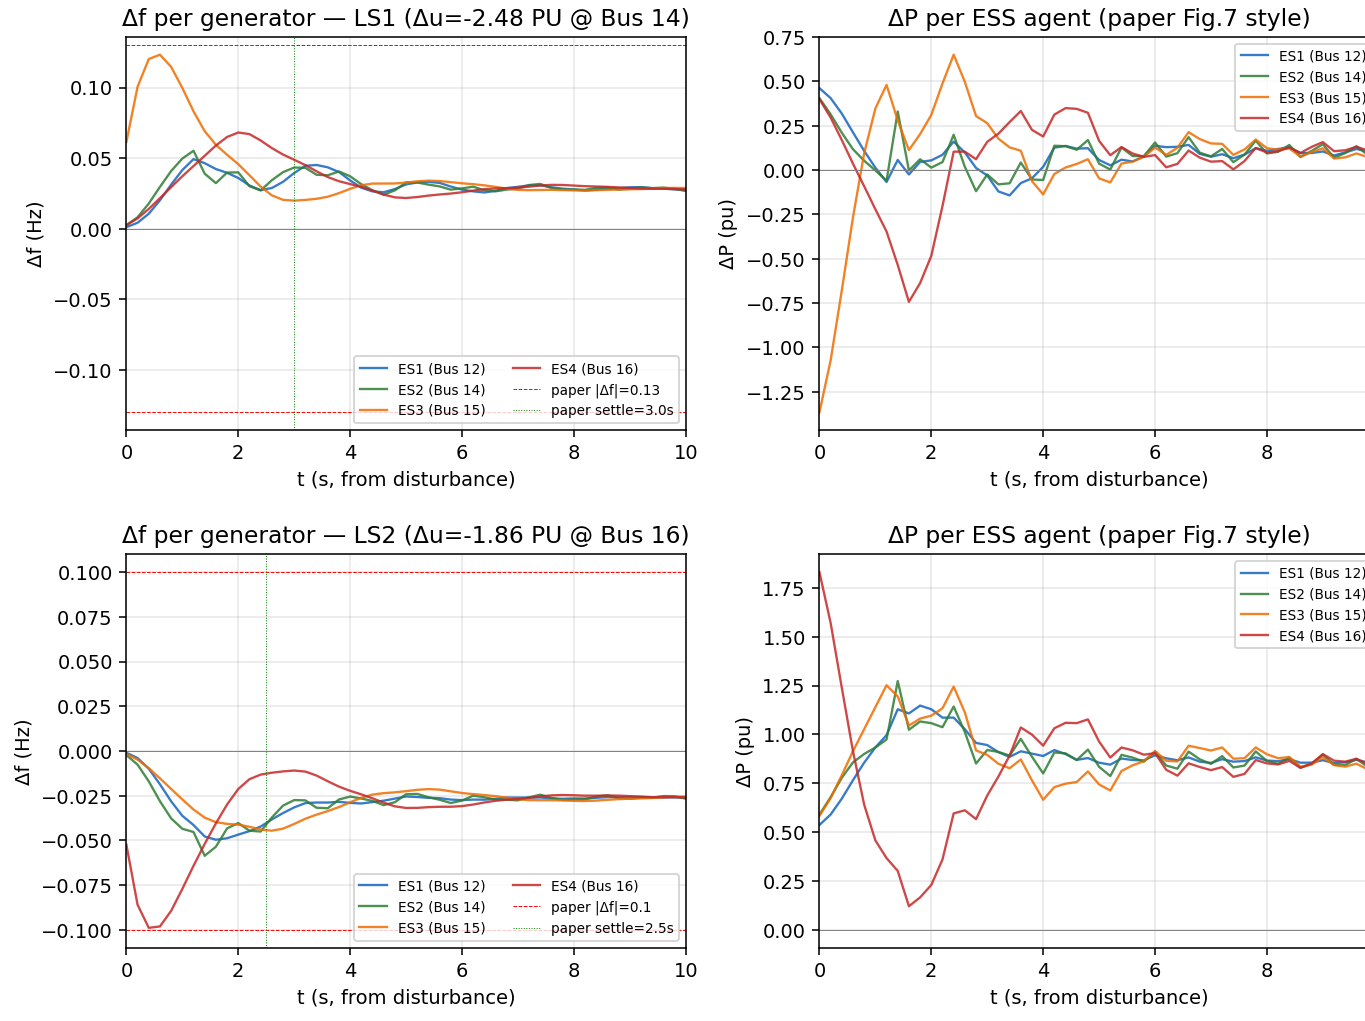
\includegraphics[width=0.95\linewidth]{proposal_control_effect}
  \caption{Closed-loop response of the canonical multi-agent controller
  (R72, eleven-axis score 0.391, four-agent power balance 0.96) under the
  two load-disturbance scenarios (LS1 top, LS2 bottom). Left: frequency
  deviation $\Delta f$ at the four machines; right: active-power
  adjustment $\Delta P$ at the four energy-storage VSG agents. The
  frequencies return toward nominal within a few seconds and track the
  reference paper's response (dashed line). Author's own work.}
  \label{fig:control}
\end{figure}

% =====================================================================
\section{Proposed Research and Methodology}

\subsection{Aim and research questions}

The aim is to move multi-agent RL control of paralleled VSGs from the
strong-but-topology-bound position established above toward control that
is transferable and deployable. Three research questions arise from those findings:

\begin{description}
  \item[RQ1 (Necessity).] Under what disturbance and operating
        conditions does learning-based control improve on a well-tuned
        classical adaptive-droop controller by a margin that justifies
        its cost, and when is classical control the rational choice?
  \item[RQ2 (Limitations).] What are the structural limits of
        per-topology RL agents: the sample cost, the single-network
        specificity, and the act-and-hold saturation mechanism
        identified in the preliminary work?
  \item[RQ3 (Topology-general deployability, core).] Can a
        graph-neural-network policy, which ingests the power network as a
        graph, be trained to coordinate VSGs across different grid
        topologies without per-network retraining?
        This is the central obstacle to industrial use.
\end{description}

These three questions set the agenda the applicant proposes to pursue;
their precise formulation, and the balance among them, will be developed
with the supervisor as the work matures, in keeping with the exploratory
nature of a research degree.

\subsection{Methodology and research approach}

The work is computational and draws on three information sources: the
ANDES phasor-domain simulator~\cite{cui2021andes}, which generates the
time-domain frequency responses used for training and evaluation; the
VSG-control, RL, and GNN literature; and the applicant's own audited
experimental ledger, which supplies verified baselines and guards
against regression.

The study will use a set of benchmark
topologies: the modified Kundur four-machine system (Figure~\ref{fig:kundur})
as the
anchor, augmented with additional standard test networks of differing
size and structure. Training on a subset and testing on held-out
topologies is how transfer will be measured. The advantage is direct relevance to
the deployment question; the cost is the effort of building and
calibrating several simulated networks, which is scoped as core work for
the degree.

\begin{figure}[t]
  \centering
  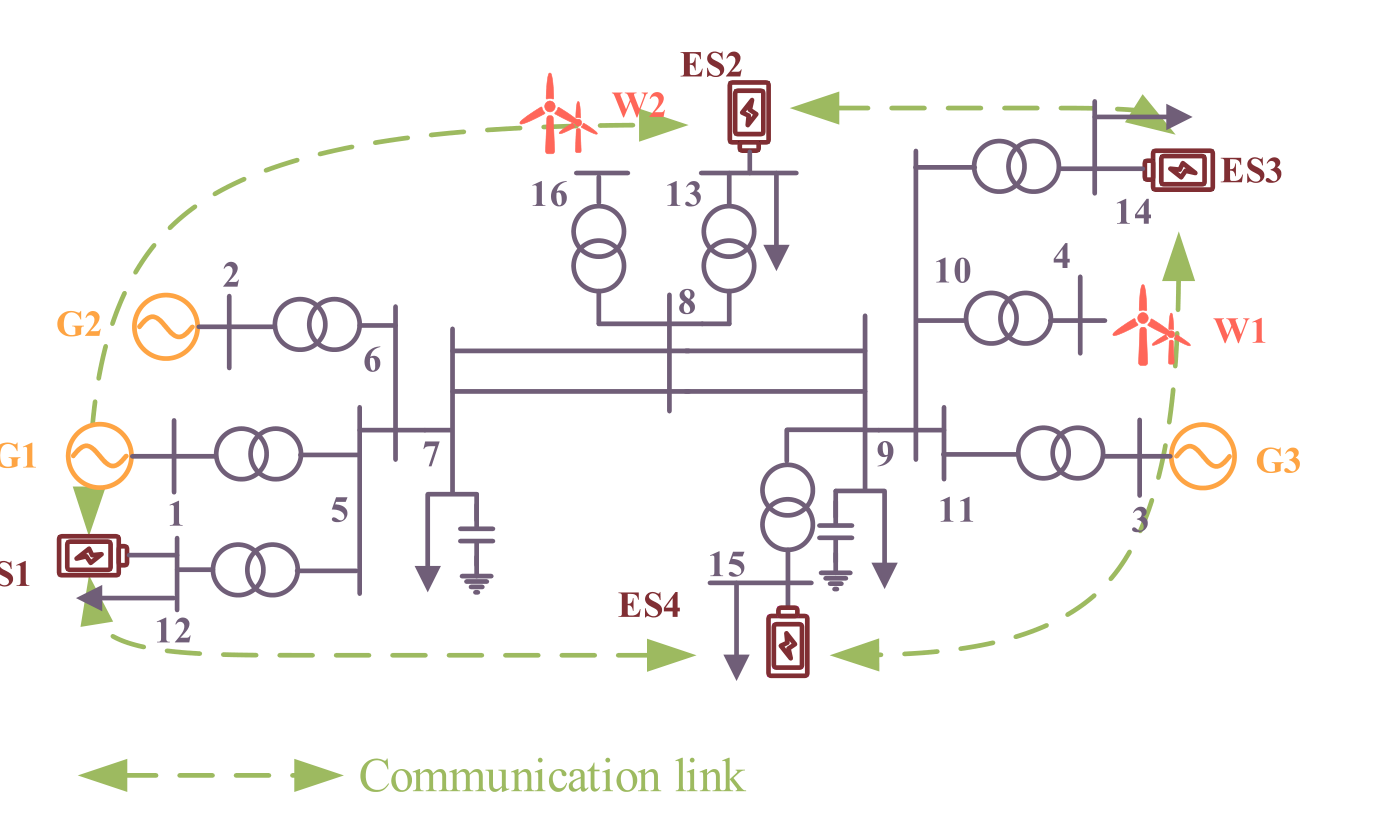
\includegraphics[width=0.86\linewidth]{paper_fig3_kundur}
  \caption{The modified Kundur two-area test system: synchronous
  generators G1--G3, four energy-storage VSG units (ES1--ES4), wind
  sources (W1--W2), and the inter-agent communication links. This is the
  anchor network on which the controllers are trained and evaluated, to
  be augmented with further topologies to test cross-network transfer.
  Source: Yang \emph{et al.}~\cite{yang2023ddic}.}
  \label{fig:kundur}
\end{figure}

The objects under control are the paralleled
VSG units and the multi-agent GNN policy that sets their virtual inertia
and damping. VSGs are the appropriate subject because they are the locus
at which synthetic inertia and damping are delivered in an
inverter-dominated grid, and their cross-topology coordination is the
open problem that fixed-network studies cannot address.

The established ANDES testbed and the
eleven-axis, multi-seed evaluation protocol extend to multiple
topologies. A GNN-based multi-agent policy will be trained across a
family of networks, then evaluated for zero- or few-shot transfer to
held-out topologies, and benchmarked against both a tuned classical
droop controller (RQ1) and a conventional per-topology RL agent
(RQ2/RQ3). Each headline number is reported over a distribution of
random seeds, so every claim rests on a reproducible result. The
programme is scoped in three phases over the degree: locating the
necessity boundary against classical droop (RQ1), quantifying the
limits of per-topology agents (RQ2), and building and testing the
cross-topology GNN policy (RQ3).

\subsection{Rationale for the application}

This research continues work already begun under the intended
supervisor's guidance, on an established codebase, evaluation
methodology, and experimental record. The MRes provides the supervision,
time, and resources to convert a mature exploratory programme into
rigorous, publishable research on the deployability question, and is the
reason the applicant wishes to undertake this degree at the University
of Nottingham Ningbo China.

% =====================================================================
\section{Anticipated Contribution}

The research offers three contributions. The first is a
topology-general, GNN-based multi-agent controller for VSG inertia and
damping support that transfers across grid configurations without
per-network retraining, the principal obstacle to deploying
learning-based VSG control. The second is a cost--benefit account of
when learning-based control justifies its complexity over well-tuned
classical methods, which existing studies rarely provide. The third is
a reproducible, multi-dimensional evaluation framework, developed in
response to the documented reproducibility shortcomings of deep
RL~\cite{henderson2018deepreinforcement,agarwal2021precipice} and extended
here to the cross-topology setting. All three address a practical
deployment question for future low-inertia grids, where grid codes
require fast frequency response~\cite{entsoe_rfg} and the safety of
autonomous adaptive control remains open~\cite{garcia2015safe}.

% =====================================================================
\bibliographystyle{ieeetr}
\bibliography{refs}

\end{document}
